\documentclass[a4paper]{article}
\usepackage[T1,T2A]{fontenc}
\usepackage[utf8]{inputenc}
\usepackage[english,russian]{babel}
\usepackage{booktabs}
\usepackage{color,colortbl}
%\usepackage{amsmath}
%\usepackage{amsfonts}
%\usepackage{amssymb}
%\usepackage{makeidx}
% далее идёт преамбула
\usepackage{tikz}
\usetikzlibrary{graphs}

\definecolor{darkishgreen}{RGB}{39,203,22}
\definecolor{LightCyan}{rgb}{0.88,1,1}
\definecolor{Gray}{gray}{0.9}
\definecolor{lightRed}{RGB}{230,170,150}
\definecolor{modRed}{RGB}{230,82,90}
\definecolor{strongRed}{RGB}{230,6,6}

\usepackage[english,russian]{babel}

\begin{document}

\section{Информационные процессы и технологии.}

\subsection{Введение}
\textbf{Информационные технологии} - это процессы, методы поиска, сбора, хранения, обработки, предоставления, распространения информации и способы осуществления таких процессов и методов.

Информационные технологии охватывают все ресурсы,
необходимые для управления информацией, особенно компьютеры,
программное обеспечение и сети, необходимые для создания, хранения, управления, передачи и поиска информации.
Информационные технологии могут быть сгруппированы
следующим образом:
\begin{itemize}
    \item технические средства
    \item коммуникационные средства
    \item организационно-методическое обеспечение
    \item стандартизация
  \end{itemize}

Прежде всего определим что такое вычислительная машна (ЭВМ). Интуитивно понятно, что это средство для автоматизации вычислений. Однако вычислительные машины используются настолько широко что по неволе возникает сомнение в правильности интуитивного определения.

В ``Толковом словаре по информатике'' приведено следующее определение: ЭВМ --- это комплекс технических, аппаратных и программных средств, предназначенных для автоматической обработки информации, вычислений, автоматического управления. Таким образом, понятие ЭВМ тесно связано с понятиями ``информация'', ``вычисления'', ``алгоритмическая обработка''.

Объект передачи и преобразования в вычислительных системах --- \textit{информация}. Все процессы, происходящие в вычислительной системе, связаны непосредственно с различными физическими носителями информации, и все узлы и блоки этой системы явлются физической средой, в которой осуществляются информационные процессы. Информационные процессы состоят не только в передаче, но и в переобразовании, переработке и хранении информации. Все это состовляет предмет науки информатики. \textbf{Информатика} состоит из трех составных частей:
\begin{itemize}
  \item теории передачи и преобразования информации;
  \item алгоритмических средств обработки информации;
  \item вычислительных средств;
\end{itemize}

\subsection{Информационные процессы}

В ходе информационного процесса данные преобразуются из одного вида в другой с помощью методов. Обработка данных включает в себя множество различных операций. В структуре возможных операций с данными можно выделить основыне:

\begin{itemize}
\item сбор данных – накопление данных с целью обеспечения достаточной полноты информации для принятия решения;

\item формализация данных – приведение данных, поступающих из разных источников, к одинаковой форме, чтобы сделать их сопоставимыми между собой, то есть повысить их уровень доступности;

\item фильтрация данных – отсеивание «лишних» данных, в которых нет необходимости для принятия решений; при этом должен уменьшаться уровень «шума», а достоверность и адекватность данных должны возрастать;

\item сортировка данных – упорядочение данных по заданному признаку с целью удобства использования; повышает доступность информации;

\item группировка данных – объединение данных по заданному признаку с целью повышения удобства использования; повышает доступность информации;

\item архивация данных – организация хранения данных в удобной и легкодоступной форме; служит для снижения экономических затрат на хранение данных и повышает общую надежность информационного процесса в целом;

\item защита данных – комплекс мер, направленных на предотвращение утраты, воспроизведение и модификации данных;

\item транспортировка данных – прием и передача (доставка и поставка) данных между удаленными участниками информационного процесса; при этом источник данных в информатике принято называть сервером, а потребителя – клиентом;

\item преобразование данных – перевод данных из одной формы в другую или из одной структуры в другую. Пример: изменение типа носителя; книги – бумага, электронная форма, микрофотоплёнка. Необходимость в многократном преобразовании данных возникает также при их транспортировке, особенно если она осуществляется средствами, не предназначенными для транспортировки данного вида данных.

\end{itemize}

\subsection{Цифровое представление данных}

Для автоматизации работы с данными, относящимися к различным типам, очень важно унифицировать их форму представления — для этого обычно используется прием кодирования, то есть выражение данных одного типа через данные другого типа. Естественные человеческие языки --- это не что иное, как системы кодирования понятий для выражения мыслей посредством речи. К языкам близко примыкают азбуки (системы кодирования компонентов языка с помощью графических символов). Та же проблема универсального средства кодирования достаточно успешно реализуется в отдельных отраслях техники, науки и культуры. В качестве примеров можно привести систему записи математических выражений, телеграфную азбуку, морскую флажковую азбуку, систему Брайля для слепых и многое другое.

В вычислительной технике используется двоичная система кодирования, основанная на предствалении данных последовательностью всего двух знкаов: 0 и 1. Эти знаки называются двоичными цифрами (binary digit) --- или битом (bit). Особенность этой системы то что она является \textit{простейшей} из всех возможных систем счисления, если мы захотим еще упростить нам придется оставить только 0, а он сам по себе не представляет никакой информации.

Одним битом могут быть выражены два понятия: О или 1 (да или нет, черное или белое, истина или ложь и т. п.). Если количество битов увеличить до двух, то уже можно выразить четыре различных понятия:
$00 01 10 11$
Тремя битами можно закодировать восемь различных значений:
$000 001 010 011 100 101 110 111$
Увеличивая на единицу количество разрядов в системе двоичного кодирования, мы увеличиваем в два раза количество значений, которое может быть выражено в данной системе, то есть общая формула имеет вид:
$$N=2^{m}$$
где:
N --- количество независимых кодируемых значений;
m --- разрядность двоичного кодирования, принятая в данной системе.

Целые числа кодируются двоичным кодом достаточно просто — достаточно взять целое число и делить его пополам до тех пор, пока в остатке не образуется ноль или единица. Совокупность остатков от каждого деления, записанная справа налево вместе с последним остатком, и образует двоичный аналог десятичного числа.
$$19:2 = 9+1$$
$$9 : 2 = 4 + 1$$
$$4 : 2 = 2 + 0$$
$$2:2 = 1$$
Таким образом, $19_{10} = 1011_{2}$
Для кодирования целых чисел от О до 255 достаточно иметь 8 разрядов двоичного кода (8 бит). Шестнадцать бит позволяют закодировать целые числа от О до 65535, а 24 бита — уже более 16,5 миллионов разных значений.

Для кодирования действительных чисел используют 80-разрядное кодирование. При этом число предварительно преобразуется в \textit{нормализованную форму}:
$$3,1415926 = 0,31415926*10^{1}$$
$$300 000 = 0,3*10^{6}$$
$$123 456 789 = 0,123456789*10^{10}$$
Первая часть числа называется мантиссой, а вторая ---характеристикой. Большую часть из 80 бит отводят для хранения мантиссы (вместе со знаком) и некоторое фиксированное количество разрядов отводят для хранения характеристики (тоже со знаком).

\subsubsection{Кодирование текстовых данных}

Если каждому символу алфавита сопоставить определенное целое число (например, порядковый номер), то с помощью двоичного кода можно кодировать и текстовую информацию. Восьми двоичных разрядов достаточно для кодирования 256 различных символов. Этого хватит, чтобы выразить различными комбинациями восьми битов все символы английского и русского языков, как строчные, так и прописные, а также знаки препинания, символы основных арифметических действий и некоторые общепринятые специальные символы, например символ «§».
Технически это выглядит очень просто, однако всегда существовали достаточно веские организационные сложности. В первые годы развития вычислительной техники они были связаны с отсутствием необходимых стандартов, а в настоящее время вызваны, наоборот, изобилием одновременно действующих и противоречивых стандартов. Для того чтобы весь мир одинаково кодировал текстовые данные, нужны единые таблицы кодирования, а это пока невозможно из-за противоречий между символами национальных алфавитов, а также противоречий корпоративного характера. Для английского языка, захватившего де --- факто нишу международаого средства общения, противоречия уже сняты. Институт стандартизации США (ANSI — American National Standard Institute) ввел в действие систему кодирования ASCII (American Standard Code for Information Interchange — стандартный код информационного обмена США). В системе ASCII закреплены две таблицы кодирования --- базовая и расширенная. Базовая таблица закрепляет значения кодов от О до 127, а расширенная относится к символам с номерами от 128 до 255.

Первые 32 кода базовой таблицы, начиная с нулевого, отданы производителям аппаратных средств (в первую очередь производителям компьютеров и печатающих устройств). В этой области размещаются так называемые управляющие коды, которым не соответствуют никакие символы языков, и, соответственно, эти коды не выводятся ни на экран, ни на устройства печати, но ими можно управлять тем, как производится вывод прочих данных.

Аналогичные системы кодирования текстовых данных были разработаны и в других странах. Так, например, в СССР в этой области действовала система кодирования КОИ-7 (код обмена информацией, семизначный). Однако поддержка производителей оборудования и программ вывела американский код ASCII на уровень международного стандарта, и национальным системам кодирования пришлось «отступить» во вторую, расширенную часть системы кодирования, определяющую значения кодов со 128 по 255 Отсутствие единого стандарта в этой области привело к множественности одновременно действующих кодировок. Только в России можно указать три действующих стандарта кодировки и еще два устаревших. Так, например, кодировка символов русского языка, известная как кодировка Windows-1251 у была введена «извне» — компанией Microsoft, но, учитывая широкое распространение операционных систем и других продуктов этой компании в России, она глубоко закрепилась и нашла широкое распространение. Эта кодировка используется на большинстве локальных компьютеров, работающих на
платформе Windows.

Если проанализировать организационные трудности, связанные с созданием единой системы кодирования текстовых данных, то можно прийти к выводу, что они вызваны ограниченным набором кодов (256). В то же время очевидно, что если, например, кодировать символы не восьмиразрядными двоичными числами, а числами с большим количеством разрядов, то и диапазон возможных значений кодов станет намного больше. Такая система, основанная на 16-разрядном кодировании символов, получила HdiSBdiiine универсальной — UNICODE. Шестнадцать разрядов позволяют обеспечить уникальные коды для 65 536 различных символов — этого поля достаточно для размещения в одной таблице символов большинства языков планеты. Несмотря на тривиальную очевидность такого подхода, простой механический переход на данную систему долгое время сдерживался из-за недостаточных ресурсов средств вычислительной техники (в системе кодирования UNICODE все текстовые документы автоматически становятся вдвое длиннее). Во второй половине 90-х годов технические средства достигли необходимого уровня обеспеченности ресурсами, и сегодня мы наблюдаем постепенный перевод документов и программных средств на универсальную систему кодирования. Для индивидуальных пользователей это еще больше добавило забот по согласованию документов, выполненных в разных системах кодирования, с программными средствами, но это надо понимать как трудности переходного периода. В настоящее время стандарт является преобладающим в Интернете.

\subsubsection{Кодирование графических данных}

Если рассмотреть с помощью увеличительного стекла черно-белое графическоеизображение, напечатанное в газете или книге, то можно увидеть, что оно состоит из мельчайших точек, образующих характерный узор, называемый растром.

Поскольку линейные координаты и индивидуальные свойства каждой точки (яркость) можно выразить с помощью целых чисел, то можно сказать, что растровое кодирование позволяет использовать двоичный код для представления графических данных. Общепринятым на сегодняшний день считается представление черно-белых иллюстраций в виде комбинации точек с 256 градациями серого цвета, и, таким образом, для кодирования яркости любой точки обычно достаточно восьмиразрядного двоичного числа. Для кодирования цветных графических изображений применяется принцип декомпозиции произвольного цвета на основные составляющие. В качестве таких составляющих используют три основные цвета: красный (Red, R), зеленый (Green, G) и синий (Blue, В). На практике считается (хотя теоретически это не совсем так), что любой цвет, видимый человеческим глазом, можно получить путем механического смешения этих трех основных цветов. Такая система кодирования называется системой RGB по первым буквам названий основных цветов.

Если для кодирования яркости каждой из основных составляющих использоватьпо 256 значений (восемь двоичных разрядов), как это принято для полутоновых черно-белых изображений, то на кодирование цвета одной точки надо затратить 24 разряда. При этом система кодирования обеспечивает однозначное определение 16,5 млн различных цветов, что на самом деле близко к чувствительности человеческого глаза. Режим представления цветной графики с использованием 24 двоичных разрядов называется полноцветным (True Color).

Каждому из основных цветов можно поставить в соответствие дополнительный цвет, то есть цвет, дополняющий основной цвет до белого. Нетрудно заметить, что для любого из основных цветов дополнительным будет цвет, образованный суммой пары остальных основных цветов. Соответственно, дополнительными цветами являются: голубой (Cyan, С), пурпурный (Magenta, М) и желтый ( Yellow, У). Принцип декомпозиции произвольного цвета на составляющие компоненты можно применять не только для основных цветов, но и для дополнительных, то есть любой цвет можно представить в виде суммы голубой, пурпурной и желтой составляющей. Такой метод кодирования цвета принят в полиграфии, но в полиграфии используетсяеще и четвертая краска — черная (Black, К). Поэтому данная система кодировани обозначается четырьмя буквами СМYK (цвет черный обозначается буквой К, потому,
что буква В уже занята синим цветом), и для представления цветной графики в этой системе надо иметь 32 двоичных разряда. Такой режим тоже называется полноцветным (true Color).

Если уменьшить количество двоичных разрядов, используемых для кодирования цвета каждой точки, то можно сократить объем данных, но при этом диапазон кодируемых цветов заметно сокращается. Кодирование цветной графики 16-разрядными двоичными числами называется режимом High Color.

При кодировании информации о цвете с помощью восьми бит данных можно передать только 256 цветовых оттенков. Такой метод кодирования цвета называется индексным. Смысл названия в том, что, поскольку 256 значений совершенно недостаточно, чтобы передать весь диапазон цветов, доступный человеческому глазу, код каждой точки растра выражает не цвет сам по себе, а только его номер (индекс) в некоей справочной таблице, называемой палитрой. Разумеется, эта палитра должна прикладываться к графическим данным — без нее нельзя воспользоваться методами воспроизведения информации на экране или бумаге (то есть, воспользоваться, конечно. можно, но из-за неполноты данных полученная информация не будет адекватной: листва на деревьях может оказаться красной, а небо — зеленым).

\subsubsection{Кодирование звуковой информации}

Приемы и методы работы со звуковой информацией пришли в вычислительную технику наиболее поздно. К тому же, в отличие от числовых, текстовых и графических данных, у звукозаписей не было столь же длительной и проверенной истории кодирования. В итоге методы кодирования звуковой информации двоичным кодом далеки от стандартизации. Множество отдельных компаний разработали свои корпоративные стандарты, но если говорить обобщенно, то можно выделить два основных направления. Метод FM (Frequency Modulation) основан на том, что теоретически любой сложный
звук можно разложить на последовательность простейших гармонических сигналов разных частот, каждый из которых представляет собой правильную синусоиду, а следовательно, может быть описан числовыми параметрами, то есть кодом. В природе звуковые сигналы имеют непрерывный спектр, то есть являются аналоговыми. Их разложение в гармонические ряды и представление в виде дискретных цифровых сигналов выполняют специальные устройства — аналогово-цифровые преобразователи (АЦП). Обратное преобразование для воспроизведения звука, закодированного числовым кодом, выполняют цифро-аналоговые преобразователи (ЦАП). При таких преобразованиях неизбежны потери информации, связанные с методом кодирования, поэтому качество звукозациси обычно получается не вполне удовлетворительным и соответствует качеству звучания простейших электромузыкальных инструментов с окрасом, характерным для электронной музыки. В то же время, данный метод кодирования обеспечивает весьма компактный код, и потому он нашел
применение еще в те годы, когда ресурсы средств вычислительной техники были явно недостаточны.

Метод таблично-волнового (Wave-Table) синтеза лучше соответствует современному уровню развития техники. Если говорить упрощенно, то можно сказать, что где-то в заранее подготовленных таблицах хранятся образцы звуков для множества различных музыкальных инструментов (хотя не только для них). В технике такие образцы
называют сэмплами. Числовые коды выражают тип инструмента, номер его модели, высоту тона, продолжительность и интенсивность звука, динамику его изменения, некоторые параметры среды, в которой происходит звучание, а также прочие параметры, характеризующие особенности звука. Поскольку в качестве образцов используются «реальные» звуки, то качество звука, полученного в результате синтеза, получается очень высоким и приближается к качеству звучания реальных музыкальных инструментов.




\subsection{Позиционные системы счисления.}

Под системой счисления принято понимать совокупность приемов записи чисел. Условные знаки, которые при этом применяются, называют цифрами. В некоторых системах счисления кроме цифр могут использоваться специальные символы. Таким образом, в системах счисления числа записываются как последовательность цифр или специальных символов. Системы счисления подразделяются на позиционные и непозиционные. В непозиционной системе счисления значение цифры не зависит от ее положения в записи числа. К непозиционной системе счисления относится, так называемая, Римская система счисления. Например, возьмем число XXX из Римской системы счисления. В данном числе цифра X в любом месте означает число десять. В позиционных системах счисления значение каждой цифры зависит от ее положения (позиции) в ряду цифр, изображающих это число. Например. В числе 999 (десятичная система счисления) первая справа цифра 9 означает количество единиц, содержащихся в числе, вторая - количество десятков, третья - количество сотен. Принимая за основание системы различные числа можно получить соответствующие системы счисления. Число Рединиц одного разряда, объединяемых в единицу более старшего разряда, называют основанием позиционной системы счисления, а сама система называется Р-ичной. Поэтому для записи произвольного числа в какой-либо позиционной системе счисления достаточно иметь Р различных цифр. Таким образом, любая позиционная система с любым целым основанием P (при P>1) использует Р различных цифр а, которые обозначают последовательный ряд чисел от 0 и кончая числом Р-1.

Число записывается в виде последовательности Р-ичных цифр, которая разделена точкой на целую и дробную части. Если каждый из символов $а_{n}, a_{n-1},\dots,a_{1}, a_{0}, a_{-1}, \dots,a_{m}$ означает некоторую Р-ичную цифру, то запись числа имеет вид $а_{n}, a_{n-1},\dots,a_{1}, a_{0},a_{-1}, \dots,a_{m}$. Каждой цифре из этой последовательности принято определенное значение. Цифра, стоящая в некотором разряде, имеет значение в Р раз большее того, которое она имела бы в разряде с номером, меньшим на
1. И наоборот, в Р раз меньше того, которое она имела бы в разряде с номером, большим на 1.

Как было сказано, количество различных цифр, применяемых в позиционной системе счисления, называют ее основанием. Принимая за основание системы различные числа можно получить соответствующие системы счисления. К позиционной системе счисления, получившим наибольшее распространение, относятся десятичная, двоичная, восьмеричная и шестнадцатеричная системы счисления. Для того, чтобы отличать в какой системе представлено то или иное число, в дальнейшем будем записыватьчисло с указанием используемой системы счисления. Например, $375_{10}$ - число 375 в десятичной системе счисления, а число $375_{8}$ - число 375 в восьмеричной системе счисления.

\textbf{Десятичная система счисления}

Это наиболее широко распространенная система счисления, которая использует 10 различных базисных цифр для представления любой величины. При записи чисел в десятичной системе счисления используются символы 0, 1, 2, 3, 4, 5, 6, 7, 8, 9.

Несмотря на простоту и привычность десятичной системы счисления, использование ее при передачи информации в вычислительных машинах представляется неудобной и технически не экономичной. Поэтому при организации вычислительных процессов в ЭВМ используются системы счисления с другими основаниями.

\textbf{Двоичная система счисления}

Большинство элементов, из которых строится ЭВМ, по своей физической природе могут находиться лишь в одном из двух состояний. Такие элементы называются двухпозиционными. Одно из устойчивых состояний элемента принимается за изображение цифры 0, а другое за изображение цифры 1. С помощью двухпозиционных элементов легко изображаются разряды двоичного числа. Поэтому двоичная система счисления имеет преимущества, и она оказывается очень удобной для применения в ЭВМ. Двоичная система счисления имеет только две цифры: 0 и 1. Это минимальное количество цифр, которое может быть принято в системе счисления. Как и в десятичной системе счисления, в двоичной системе для отделения дробной части от целой используется точка, а перед отрицательным числом ставиться минус (-): $101.1_{2}, 1.001_{2}, -101_{2}$.

\textbf{Восьмеричная система счисления}

В цифровых схемах и электронных системах получила распространение восьмеричная система счисления. Данная система удобна тем, что восьмеричная запись какого-либо числа в три раза короче его двоичной записи. В данной системе счисления коэффициенты принимают восемь различных значений - 0, 1, 2, 3, 4, 5, 6, 7.
Поэтому каждый восьмеричный символ может быть представлен трехбитовым числом. Этих чисел восемь, как и символов в восьмеричной системе счисления. Как и в рассмотренных системах счисления, в восьмеричной системе используются дробные и отрицательные числа: $7.35_{8},- 5.001_{8}, 345.67_{8}$.

\textbf{Шестнадцатеричная система счисления}

Для систем счисления с основанием больше «10», арабских цифр для представления чисел не хватит. Поэтому в этих случаях дополнительно вводят специальные символы. К таким системам счисления относится шестнадцатеричная система счисления.В шестнадцатеричной системе счисления используют 16 базисных символов: 0, 1, 2, 3, 4, 5, 6, 7, 8, 9, А, В, С, D, Е, F. Выбор шестнадцатеричной системы счисления обуславливается что эту систему можно использовать как средство сокращенной записи четырехзначного двоичного числа. Следует помнить, что шестнадцатеричные и восьмеричные числа - это только способ представления двоичных чисел. Для представления дробных чисел и отрицательных шестнадцатеричных чисел используется, соответственно, точка и знак минуса (-): $-AB_{16}; 1036.F_{16};FF.13_{16}$.

\textbf{Перевод чисел в позиционных системах счисления}

Для перевода целого десятичного числа в другую систему счисления, необходимо разделить исходное число на основание системы счисления, в которое оно переводится. При этом надо определять остатки от деления. Остаток первого деления является значением младшего разряда. Затем полученное частное делится на выбранное основание. Процедуру деления продолжают до тех пор, пока частное не станет меньше делителя, т.е. основания системы счисления, в которую осуществляется перевод. Значение последнего частного будет наибольшим разрядом, т.е. запись нового числа производится в обратном порядке: от частного к первому остатку,y используя все промежуточные остатки. При переводе в шестнадцатеричную систему счисления остатки, значения которых больше 9, необходимо заменить соответствующими буквенным эквивалентом: 10 - А, 11 - В, 12 - С, 13 - D, 14 -Е, 15 -F.

Пример перевода десятичного числа 95:

В двоичную систему счисления $95_{10}=1011111_{2}$
\begin{figure}[h]
\center{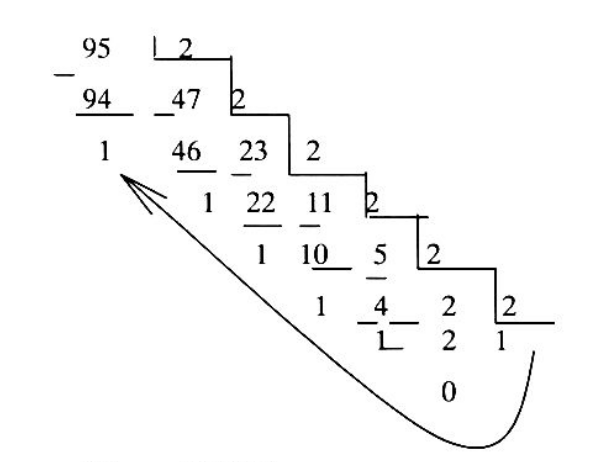
\includegraphics[width=128pt]{dectobin.png}
\label{ris:dectooct}}
\end{figure}


В восьмиричную систему счисления $95_{10}=137_{8}$
\begin{figure}[h]
\center{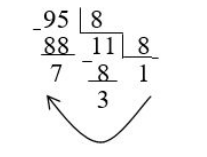
\includegraphics[width=64pt]{dectooct.png}
  \label{ris:dectooct}}
\end{figure}

В шестнадцатиричную систему счисления $95_{10}=5F_{16}$
\begin{figure}[h]
\center{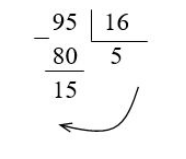
\includegraphics[width=64pt]{dectohex.png}
  \label{ris:dectohex}}
\end{figure}

При переводе правильных десятичных дробей, необходимо умножить значение этой дроби на основание системы счисления, в которую осуществляется перевод. Значение целой части результата первого умножения присваивается старшему разряду дробной части. Затем целая часть не рассматривается и производится следующее умножение дробной части. Процедуру умножения повторяют до тех пор, пока результат умножения не будет равен целому числу и этот результат будет младшим разрядом, либо не будет достигнута требуемая точность.

Пример перевода десятичного числа 0.36:

В двоичную систему счисления $0.36_{10}=0.0101_{2}$
\begin{figure}[h]
\center{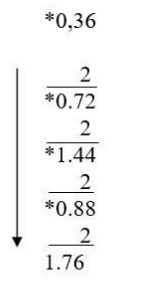
\includegraphics[width=64pt]{fdectobin.png}
  \label{ris:fdectobin}}
\end{figure}

В восьмиричную систему счисления $0.36_{10}=0.2702_{8}$

\begin{figure}[h]
\center{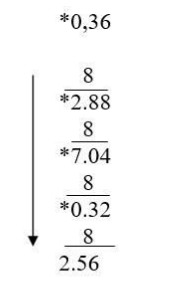
\includegraphics[width=64pt]{fdectooct.png}
  \label{ris:fdectooct}}
\end{figure}

В шестнадцатиричную систему счисления $0.36_{10}=0.5C28_{16}$

\begin{figure}[h]
\center{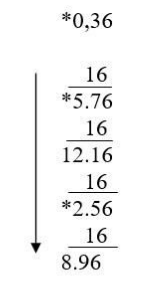
\includegraphics[width=64pt]{fdectohex.png}
  \label{ris:fdectohex}}
\end{figure}

Для перевода неправильной десятичной дроби, необходимо перевести отдельно дробную и целую часть, а полученные результаты сложить. Например, перевести в двоичную систему счисления неправильную десятичную дробь 14.375.
$$14_{10}=1110_{2} 0.375_{10}=0.011_{2} 14.375_{10}=1110.011_{2}$$

\textbf{Перевод в десятичную систему счисления}
Для перевода из любой позиционной системы счисления в десятичную систему счисления необходимо записать это число в виде суммы:
$$x = \sum^{n+m}_{i=1}(a_{i}*p^{n-i})$$
где Р --- основание системы из которой осуществляется перевод;\newline
а --- число, соответствующее базисной цифре Р-ичной системы счисления;\newline
n --- число цифр в целой части, m - число цифр в дробной части.\newline
Например, перевести число $110.101_{2}$ из двоичной системы счисления в десятичную:
$$110.101_{2} = 1 * 2^{2} + 1 * 2^{1} + 0 + 1 * 2^{-2} + 1 * 2^{-3} = 6.625_{10}$$

\textbf{Перевод из двоичной системы счисления в восьмеричную и шестнадцатеричную}

Основания восьмеричной и шестнадцатеричной систем счисления (q) являются степенью двоичной системы $(р):q=p$, где к --- целое число, равное 3 для восьмеричной системы счисления и 4 для шестнадцатеричной. Поэтому перевод из двоичной системы осуществляется разбиением двоичного числа на группы по три цифры в каждой для восьмеричной и по четыре для шестнадцатеричной. Отчет ведется от точки разделяющей целую часть от дробной в обе стороны. Затем каждая группа заменяется соответствующей цифрой из соответствующих систем счисления(см. табл. \ref{tab:octhex}). Недостающие биты двоичного числа дополняются нулями: впереди - для целой части и в конце - для дробной части. Например, необходимо перевести двоичное число 1010001110.00111 в восьмеричное и шестнадцатеричное число:
\begin{itemize}
  \item в восьмеричное $1010001110.00111_{2} = 001 010 001 100.001 110_{2} = 1214.16_{8}$
  \item в шестнадцатеричное $1010001110.00111_{2} = 0010 1000 1100.0011 1000_{2} = 28С.38_{16}$
\end{itemize}

\begin{table}[h]
  \caption{Соответствие цифр в разных системах счисления}
  \begin{center}\label{tab:octhex}
    \begin{tabular}{|c|c|c|}
      \hline
     Символы & k - 3 & k - 4 \\
     \hline
      0 & 000 & 0000 \\
      1 & 001 & 0001 \\
      2 & 010 & 0010 \\
      3 & 011 & 0011 \\
      4 & 100 & 0100 \\
      5 & 101 & 0101 \\
      6 & 110 & 0110 \\
      7 & 111 & 0111 \\
      8 &     & 1000 \\
      9 &     & 1001 \\
      A &     & 1010 \\
      B &     & 1011 \\
      C &     & 1100 \\
      D &     & 1101 \\
      E &     & 1110 \\
      F &     & 1111 \\
      \hline
     \end{tabular}
  \end{center}
\end{table}

\textbf{Перевод в двоичную систему счисления из восьмеричной и шестнадцатеричной}
Для перевода в двоичную систему из восьмеричной или шестнадцатеричной системы счисления необходимо каждое число заменить двоичным эквивалентом (см. табл. \ref{tab:octhex}).

\textbf{Перевод из восьмеричной системы в шестнадцатеричную}
Для перевода из восьмеричной системы счисления в шестнадцатеричную систему счисления необходимо представить число в виде двоичного числа. Затем объединить в группы по 4 бита и заменить соответствующим числом из шестнадцатеричной системы счисления (см. табл. \ref{tab:octhex})

\textbf{Перевод из шестнадцатеричной системы в восьмеричную}
Для перевода из шестнадцатеричной системы счисления в восьмеричную необходимо представить число в виде двоичного числа. Затем объединить в группы по 3 бита и заменить соответствующим числом из восьмеричной системы счисления (см. табл. \ref{tab:octhex}).

\textbf{Арифметические действия в позиционных системах счисления}
Арифметические действия (сложение, вычитание, умножение и деление) над числами в восьмеричной и шестнадцатеричной системах счисления выполняются с использованием таблиц сложения и умножения подобно тому, как это делается в десятичной системе счисления. Таблицы \ref{tab:octsum} и \ref{tab:octmul} предназначены для выполнения сложения и умножения --- в восьмеричной системе счисления, а таблицы \ref{tab:hexsum} и \ref{tab:hexmul} - в шестнадцатеричной системе счисления. Ниже приведены примеры сложения и умножения в различных системах счисления.

\begin{table}[h]
  \caption{Сложение в восьмеричной системе}
  \begin{center}\label{tab:octsum}
\begin{tabular}{|c|c|c|c|c|c|c|c|}
  \hline
  + & 1 & 2 & 3 & 4 & 5 & 6 & 7\tabularnewline
\hline
1 & 2 & 3 & 4 & 5 & 6 & 7 & 10\tabularnewline
\hline
2 & 3 & 4 & 5 & 6 & 7 & 10 & 11\tabularnewline
\hline
3 & 4 & 5 & 6 & 7 & 10 & 11 & 12\tabularnewline
\hline
4 & 5 & 6 & 7 & 10 & 11 & 12 & 13\tabularnewline
\hline
5 & 6 & 7 & 10 & 11 & 12 & 13 & 14\tabularnewline
\hline
6 & 7 & 10 & 11 & 12 & 13 & 14 & 15\tabularnewline
\hline
7 & 10 & 11 & 12 & 13 & 14 & 15 & 16\tabularnewline
                                  \hline
\end{tabular}
\end{center}
\end{table}

\begin{table}[h]
  \caption{Умножение в восьмеричной системе}
  \begin{center}\label{tab:octmul}
\begin{tabular}{|c|c|c|c|c|c|c|c|}
\hline
{*} & 1 & 2 & 3 & 4 & 5 & 6 & 7\tabularnewline
\hline
1 & 1 & 2 & 3 & 4 & 5 & 6 & 7\tabularnewline
\hline
2 & 2 & 4 & 6 & 10 & 12 & 14 & 16\tabularnewline
\hline
3 & 3 & 6 & 11 & 14 & 17 & 22 & 25\tabularnewline
\hline
4 & 4 & 10 & 14 & 20 & 24 & 30 & 34\tabularnewline
\hline
5 & 5 & 12 & 17 & 24 & 31 & 36 & 43\tabularnewline
\hline
6 & 6 & 14 & 22 & 30 & 36 & 44 & 52\tabularnewline
\hline
7 & 7 & 16 & 25 & 34 & 43 & 52 & 61\tabularnewline
\hline
\end{tabular}
\end{center}
\end{table}

\begin{table}[h!]
  \caption{Сложение в шестнадцатеричной системе}
  \begin{center}\label{tab:hexsum}
\begin{tabular}{|c|c|c|c|c|c|c|c|c|c|c|c|c|c|c|c|}
\hline
+ & 1 & 2 & 3 & 4 & 5 & 6 & 7 & 8 & 9 & A & B & C & D & E & F\tabularnewline
\hline
1 & 2 & 3 & 4 & 5 & 6 & 7 & 8 & 9 & A & B & C & D & E & F & 10\tabularnewline
\hline
2 & 3 & 4 & 5 & 6 & 7 & 8 & 9 & A & B & C & D & E & F & 10 & 11\tabularnewline
\hline
3 & 4 & 5 & 6 & 7 & 8 & 9 & A & B & C & D & E & F & 10 & 11 & 12\tabularnewline
\hline
4 & 5 & 6 & 7 & 8 & 9 & A & B & C & D & E & F & 10 & 11 & 12 & 13\tabularnewline
\hline
5 & 6 & 7 & 8 & 9 & A & B & C & D & E & F & 10 & 11 & 12 & 13 & 14\tabularnewline
\hline
6 & 7 & 8 & 9 & A & B & C & D & E & F & 10 & 11 & 12 & 13 & 14 & 15\tabularnewline
\hline
7 & 8 & 9 & A & B & C & D & E & F & 10 & 11 & 12 & 13 & 41 & 15 & 16\tabularnewline
\hline
8 & 9 & A & B & C & D & E & F & 10 & 11 & 12 & 13 & 14 & 15 & 16 & 17\tabularnewline
\hline
9 & A & B & C & D & E & F & 10 & 11 & 12 & 13 & 14 & 15 & 16 & 17 & 18\tabularnewline
\hline
A & B & C & D & E & F & 10 & 11 & 12 & 13 & 14 & 15 & 16 & 17 & 18 & 19\tabularnewline
\hline
B & C & D & E & F & 10 & 11 & 12 & 13 & 14 & 15 & 16 & 17 & 18 & 19 & 1A\tabularnewline
\hline
C & D & E & F & 10 & 11 & 12 & 13 & 14 & 15 & 16 & 17 & 18 & 19 & 1A & 1B\tabularnewline
\hline
D & E & F & 10 & 11 & 12 & 13 & 14 & 15 & 16 & 17 & 18 & 19 & 1A & 1B & 1C\tabularnewline
\hline
E & F & 10 & 11 & 12 & 13 & 14 & 15 & 16 & 17 & 18 & 19 & 1A & 1B & 1C & 1D\tabularnewline
\hline
F & 10 & 11 & 12 & 13 & 14 & 15 & 16 & 17 & 18 & 19 & 1A & 1B & 1C & 1D & 1E\tabularnewline
\hline
\end{tabular}
\end{center}
\end{table}

\begin{table}[h!]
  \caption{Умножение в шестнадцатеричной системе}
  \begin{center}\label{tab:hexmul}
\begin{tabular}{|c|c|c|c|c|c|c|c|c|c|c|c|c|c|c|c|}
\hline
{*} & 1 & 2 & 3 & 4 & 5 & 6 & 7 & 8 & 9 & A & B & C & D & E & F\tabularnewline
\hline
1 & 1 & 2 & 3 & 4 & 5 & 6 & 7 & 8 & 9 & A & B & C & D & E & F\tabularnewline
\hline
2 & 2 & 4 & 6 & 8 & A & C & E & 10 & 12 & 14 & 16 & 18 & 1A & 1C & 1E\tabularnewline
\hline
3 & 3 & 6 & 9 & C & F & 12 & 15 & 18 & 1B & 1E & 21 & 24 & 27 & 2A & 2D\tabularnewline
\hline
4 & 4 & 8 & C & 10 & 14 & 18 & 1C & 20 & 24 & 28 & 2C & 30 & 34 & 38 & 3C\tabularnewline
\hline
5 & 5 & A & F & 14 & 19 & 1E & 23 & 28 & 2D & 32 & 37 & 3C & 41 & 46 & 4B\tabularnewline
\hline
6 & 6 & C & 12 & 18 & 1E & 24 & 2A & 30 & 36 & 3C & 42 & 48 & 4E & 54 & 5A\tabularnewline
\hline
7 & 7 & E & 15 & 1C & 23 & 2A & 31 & 38 & 3F & 46 & 4D & 54 & 5B & 62 & 69\tabularnewline
\hline
8 & 8 & 10 & 18 & 20 & 28 & 30 & 38 & 40 & 48 & 50 & 58 & 60 & 68 & 70 & 78\tabularnewline
\hline
9 & 9 & 12 & 1B & 24 & 2D & 36 & 3F & 48 & 51 & 5A & 63 & 6C & 75 & 7E & 87\tabularnewline
\hline
A & A & 14 & 1E & 28 & 32 & 3C & 46 & 50 & 5A & 64 & 6E & 78 & 82 & 8C & 96\tabularnewline
\hline
B & B & 16 & 21 & 2C & 37 & 42 & 4D & 58 & 63 & 6E & 79 & 84 & 8F & 9A & A5\tabularnewline
\hline
C & C & 18 & 24 & 30 & 3C & 48 & 54 & 60 & 6C & 78 & 84 & 90 & 9C & A8 & B4\tabularnewline
\hline
D & D & 1A & 27 & 34 & 41 & 4E & 5B & 68 & 75 & 82 & 8F & 9C & A9 & B6 & C3\tabularnewline
\hline
E & E & 1C & 2A & 38 & 46 & 54 & 62 & 70 & 7E & 8C & 9A & A8 & B6 & C4 & D2\tabularnewline
\hline
F & F & 1E & 2D & 3C & 4B & 5A & 69 & 78 & 87 & 96 & A5 & B4 & C3 & D2 & E1\tabularnewline
\hline
\end{tabular}
\end{center}
\end{table}


\subsection{Единицы измерения информации. Разновидности носителей информации.}

Существует много различных систем и единиц измерения данных. Каждая научная дисциплина и каждая область человеческой деятельности может использовать свои, наиболее удобные или традиционно устоявшиеся единицы. В информатике для измерения данных используют тот факт, что разные типы данных имеют универсальное двоичное представление и потому вводят свои единицы данных, основанные на нем. Наименьшей единицей измерения является байт. Поскольку одним байтом, как правило, кодируется один символ текстовой информации, то для текстовых документов размер в байтах соответствует лексическому объему в символах (пока исключение представляет рассмотренная выше универсальная кодировка ЮНИКОД). Более крупная единица измерения — килобайт (Кбайт). Условно можно считать, что 1 Кбайт примерно равен 1000 байт. Условность связана с тем, что для вьпислительной техники, работающей с двоичными числами, более удобно представление чисел в виде степени двойки и потому на самом деле 1 Кбайт равен $2^{10}байт$ (1024 байт). Однако всюду, где это не принципиально, с инженерной погрешностью (до 3\%) «забывают» о «лишних» байтах. В килобайтах измеряют сравнительно небольшие объемы данных. Условно можно считать, что одна страница неформатированного машинописного текста составляет около 2 Кбайт. Более крупные единицы измерения данных образуются добавлением префиксов мега-, гига- тера-; в более крупных единицах пока нет практической надобности.

\subsection{Еденицы хранения данных}

При хранении данных решаются две проблемы: как сохранить данные в наиболее компактном виде и как обеспечить к ним удобный и быстрый доступ (если доступ не обеспечен, то это не хранение). Для обеспечения доступа необходимо, чтобы данные имели упорядоченную структуру, а при этом, как мы уже знаем, образуется «паразитная нагрузка» в виде адресных данных. Без них нельзя получить доступ к нужным элементам данных, входящих в структуру. Поскольку адресные данные тоже имеют размер и тоже подлежат хранению, хранить данные в виде мелких единиц, таких как байты, неудабно. Их неудобно хранить и в более крупных единицах (килобайтах, мегабайтах и т. п.), поскольку неполное заполнение одной единицы хранения приводит к неэффективности хранения. В качестве единицы хранения данных принят объехсг переменной длины, называемый файлом. Файл — это последовательность произвольного числа байтов, обладаюиая уникальным собственным именем. Обычно в отдельном файле хранят данные, относящиеся к одному типу. В этом случае тип данных определяет тип файла. Проще всего представить себе файл в виде безразмерного канцелярского досье, в которое можно по желанию добавлять содержимое или извлекать его оттуда. Поскольку в определении файла нет ограничений на размер, можно представить себе файл, имеющий О байтов (пустой файл), и файл, имеющий любое число байтов. В определении файла особое внимание уделяется имени. Оно фактически несет в себе адресные данные, без которых данные, хранящиеся в файле, не станут информацией из-за отсутствия метода доступа к ним. Кроме функций, связанных с адресацией, имя файла может хранить и сведения о типе данных, заключенных в нем. Для автоматических средств работы с данными это важно, поскольку по имени файла они могут автоматически определить адекватный метод извлечения информации из файла.

\section{Архитектура ЭВМ}

\subsection{Хранение данных в памяти ЭВМ.}

Различают устройства хранения информации, реализованные в виде электронных схем, и накопители информации, при помощи которых данные записываются на какой-либо носитель, например магнитный или оптический (ранее использовались даже бумажные носители- перфокарты и перфоленты). Устройства, представляющие собой электронные схемы, отличаются небольшим временем доступа к данным, но не позволяют хранить большие объемы информации. Накопители информации наоборот дают возможность хранить большие объемы информации, но время ее записи и считывания больше.

Способы хранения битов в современных ЭВМ.Хранение бита в машине требует устройства, которое может находиться в двух состояниях, например, такого как выключатель (включен или выключен), реле (открыто или закрыто) пли флаг на флагштоке (поднят или опущен). Одно из состояний используется для обозначения 0, второе для обозначения 1.

Триггер– это схема, которая на выходе имеет значение 0 или 1, и это значение остается неизменным до тех пор, пока кратковременный импульс, исходящий от другой цепи, не заставит его переключиться на другое значение. Таким образом триггер может находиться в одном из двух состояний, одно из которых соответствует запоминанию двоичного нуля, другое — запоминанию двоичной единицы.

Современным способом хранения битов также является конденсатор, который состоит из двух небольших металлических пластин, расположенных параллельно друг другу на некотором расстоянии. Если к пластинам подсоединить источник напряжения: к одной пластине — положительный полюс, к другой — отрицательный, заряды из источника перейдут на пластины. Теперь, если убрать источник напряжения, то заряды останутся на пластинах. Если соединить пластины, то возникнет электрический ток, и заряды будут нейтрализованы. Таким образом, конденсатор может находиться в одном из двух состояний (заряжен и разряжен), одно из которых может быть принято за 0, другое — за 1. Современные технологии позволяют создать миллионы крошечных конденсаторов, объединенных в одну цепь на одной пластине (микросхеме, чипе). Поэтому конденсатор стал распространенным способом для хранения битов в машинах.

Триггеры и конденсаторы являются примерами систем хранения с различными степенями устойчивости. Триггер теряет введенные данные после отключения питания. Заряды конденсатора настолько слабы, что они имеют тенденцию рассеиваться сами по себе, даже когда машина включена. Следовательно, заряд конденсатора должен постоянно пополняться при помощи так называемой цепи регенерации. По причине этой неустойчивости память компьютера, построенная таким способом, часто называется динамической памятью.

Память.

Виды памяти показаны на слайде. Внутренняя памятьсостоит из оперативного и постоянного запоминающего устройства.

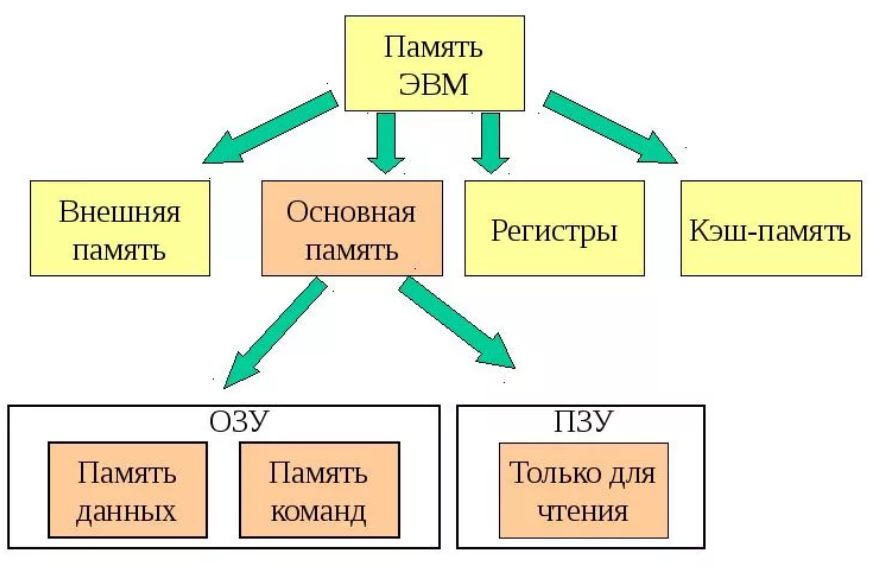
\includegraphics[width=\textwidth]{mem_l.png}

Назначение оперативной памяти – хранение данных, которые могут потребоваться в ближайшее время. В оперативное запоминающее устройство (ОЗУ), которое часто также называют оперативной памятью, с диска или дискет копируются (загружаются) программы, которые выполняются в данный момент. Это значит, что когда вы запускаете какую-либо компьютерную программу, находящуюся на диске, она копируется в оперативную память, после чего процессор начинает выполнять команды, изложенные в этой программе. Часть ОЗУ, называемая «видеопамять», содержит данные, соответствующие текущему изображению на экране. При отключении питания содержимое ОЗУ стирается. Быстродействие (скорость работы) компьютера напрямую зависит от величины его ОЗУ, которое в современных компьютерах обычно составляет Гигабайты. В первых ПК фирмы IBM (1981г.) максимальный объем оперативной памяти был равным 640 Кбайт.

Структура памяти. Запоминающие схемы в оперативной памяти компьютера объединены в управляемые единицы, называемые ячейками памяти, при этом стандартный размер ячейки равен восьми битам или одному байту. Удобно конструировать оперативную память, в которой общее число ячеек является степенью двух. Небольшие компьютеры, применяемые в такой бытовой технике, например, в микроволновой печи, могут содержать оперативную память, насчитывающую только несколько сотен ячеек, в то время как большие компьютеры, используемые для хранения и обработки огромных массивов данных, могут содержать миллиарды ячеек в своей оперативной памяти.

Соотношения между единицами измерений памяти представлено в таблице 1.2.

Таблица 1.2. Единицы измерения памяти ЭВМ.
Единица 	Содержит байт 	Содержит Кбайт 	Содержит Мбайт 	Содержит Гбайт
1байт
1Кбайт 	1024 (210)
1Мбайт 	1048576 (220)
1Гбайт 	1073741824(230)
1Тбайт

Хотя понятия «право» и «лево» не применимы по отношению к внутреннему строению машины, обычно считается, что биты внутри ячейки памяти упорядочены в строке. Последний бит левого конца называется старшим битом, так как если содержимое ячейки представляет собой число, то этот бит будет его старшим разрядом. Также бит, расположенный на правом конце, называют младшим битом.

Для того чтобы идентифицировать ячейки в оперативной памяти, каждой из них приписывается уникальное имя, которое называется адресом. Считается, что ячейки памяти расположены в ряд и пронумерованы по порядку, начиная с нуля. Такая система адресации не только позволяет единственным образом определить ячейку памяти, но также упорядочивает их, позволяя употреблять по отношению к ним такие выражения, как «следующая ячейка» или «предыдущая ячейка».

Важным следствием того, что и ячейки оперативной памяти, и биты в каждой ячейке упорядочены, является тот факт, что все биты в оперативной памяти, по существу, выстроены в длинный ряд. Следовательно, части этого ряда могут использоваться для хранения последовательностей битов, длина которых больше длины одной ячейки памяти. В частности, даже если память разделена на ячейки размером 1 байт, то мы можем хранить цепочку из 16 битов в двух последовательно расположенных ячейках.

Другим следствием представления оперативной памяти в виде упорядоченных ячеек с адресом является возможность индивидуального доступа к каждой ячейке, то есть данные, хранящиеся в оперативной памяти компьютера, могут обрабатываться в случайном порядке. Это объясняет то, что оперативную память часто называют памятью с произвольным доступом (RAM — Random Access Memory). Произвольный доступ к небольшим единицам данных (минимально это один байт) – коренное отличие оперативной памяти от устройств хранения данных, которые рассматриваются далее и в которых длинные последовательности байтов должны обрабатываться как блок. Когда оперативная память построена с использованием технологии динамической памяти (на конденсаторах), ее называют динамической памятью с произвольным доступом (DRAM - Dinamic RAM).

Для заполнения оперативной памяти схема, которая в действительности хранит биты, объединяется со схемой, необходимой для того, чтобы остальные схемы могли хранить и получать данные из ячеек памяти. Таким образом, другие схемы могут получить данные из памяти, запрашивая содержимое ячейки по определенному адресу (операцией чтения), или они могут записывать информацию в память, требуя, чтобы определенная последовательность битов была помещена в ячейку по определенному адресу (операцией записи).

Кэш память– это порция быстродействующей памяти (несколько килобайт), время отклика которой примерно равно времени отклика регистров. Часто она находится в центральном процессоре. В кэш-памяти машина хранит копию той части оперативной памяти, которая сейчас используется. При этом передача данных, которая обычно осуществляется между регистрами и оперативной памятью, происходит между регистрами и кэш-памятью. Все изменения потом передаются в оперативную память, но в более подходящее время.

Из-за зависимости от питания (обнуляется при отключении питания) и ограниченного размера оперативной памяти большинство машин снабжены устройствами хранения данных (mass storage sistem), которые включают в себя магнитные диски, компакт-диски и магнитные ленты. Основными отличиями устройств хранения данных от оперативной памяти являются их независимость от питания, большая емкость и, в большинстве случаев, автономность, то есть возможность перемещать запоминающую среду независимо от компьютера, что удобно для создания архивов.

Главным недостатком устройств хранения данных является то, что они требуют механического движения и, следовательно, обладают большим временем отклика по сравнению с оперативной памятью машины, которая является электронной.

Магнитные диски – тонкий вращающийся диск с магнитным покрытием. Запись информации на них основана на способности некоторых материалов, содержащих железо, сохранять намагниченность после кратковременного воздействия магнитного поля. Двоичные нули и единицы записываются на кольцеобразные дорожки диска в виде двух по-разному намагниченных участков. Головки чтения/записи располагаются над и/или под диском, так что, когда диск вращается, головка очерчивает кольцо на поверхности диска, называемое дорожкой. Дорожки разделены на дуги, которые называются секторами (на них информация записана в виде непрерывной последовательности битов размером 512байт). Емкость накопителя на дисках зависит от числа используемых дисков (поверхностей) и плотности расположения дорожек и секторов. Разбиение диска на дорожки и сектора называется форматированием диска.

Диски большой емкости, способные вмещать гигабайты информации, состоят из 5 – 10 жестких дисков, установленных на общем шпинделе. Устройство называется жестким диском (винчестером). Для большей скорости вращения головки чтения/записи в этих устройствах не соприкасаются с диском, а «плавают» над его поверхностью. Жесткий магнитный диск размещается внутри компьютера. Компьютер может иметь пакет (несколько) винчестеров.

Дискета представляет собой гибкий магнитный диск.

Компакт-диски – диски, состоящие из отражающего материала, покрытого прозрачным защитным слоем. Запись информации на них осуществляется посредством изменения структуры их отражающего слоя. Информация извлекается с диска при помощи лазерного луча, который контролирует отличия структуры отражающего слоя диска по мере его вращения. Информация на дисках формата CD-DA (емкость 500-700Мбайт) хранится на дорожке, похожей на спиральный желобок грампластинки. Формат DVD имеет емкость до 10Гбайт.

Магнитные ленты – информация записывается на магнитный слой тонкой пластиковой ленты, которая для хранения наматывается на бобину. Используется для автономного хранения данных (архив).

Флэш-диск – устройство хранения данных, содержащее микросхему электронной энергонезависимой памяти.

Информация на носителях хранится в виде файлов. Файл рассматривается как один многобитовый блок. Файл – область на магнитном диске, наименьшая единица хранения информации, содержащая последовательность байтов и зарегистрированная операционной системой под своим уникальным именем. Уникальное имя файла состоит из имени и расширения (типа файла). Тип файла изменить произвольно нельзя. Параметры, характеризующие файл (свойства): 1) полное имя файла; 2) объем файла в байтах; 3) дата создания файла; 4) время создания файла; 5) атрибуты файла, которые определяют степень доступа к файлу.

Логический диск - это либо весь диск, либо часть диска, предназначенная для хранения определенного объема информации. Логический диск обозначается большой латинской буквой с двоеточием. В компьютере может иметься доступ к нескольким жестким дискам, дисководам для дискет, CD-ромам. Каждый из них может представлять собой отдельный логический диск, но некоторые жесткие диски могут быть разделены на части, каждая из которых является отдельным логическим диском. Компьютер работает с каждым логическим диском как с отдельным устройством, хотя на самом деле он может представлять собой лишь часть реального (физического) диска и даже часть оперативной памяти.

Каталог (директория, англ.directory) (папка) - часть логического диска, предназначенная для хранения определенного объема информации (в виде файлов). Каталог может включать в себя несколько других каталогов (подкаталогов) и входить в состав другого каталога (надкаталога). Логический диск также является каталогом самого высокого уровня - корневым каталогом. Таким образом, на диске образуется система каталогов, имеющая древовидную (иерархическую) структуру.

Структура обработки информации на ЭВМ выглядит следующим образом. При вводе она кодируется единицами и нулями, т.е. битами, затем обрабатывается байтами. Если необходимо сохранить информацию – она «упаковывается» в файлы. При обращении к файлам происходит обратный процесс перехода от кодовой формы к естественной и понятной нам (декодирование информации).

\subsection{Язык запросов поисковиков}

Язык запросов поисковой системы – это набор операторов, на основе которых строятся правила для алгоритма поиска.

Правильно указанная шаблонизированная фраза позволяет сократить в результатах выдачи количество ссылок на сайты, не отвечающие запросу пользователя.

Вспомните столы справок в торговых центрах или на вокзалах. Все сотрудницы делятся на две категории:

    Милые приветливые девушки, терпеливо уточняющие ваш вопрос и искренне желающие помочь.
    Закаленные в боях с клиентами суровые женщины со стальным стержнем, которые выдают информацию строго в соответствии с тем, что вы спросите. И не важно, что желает узнать посетитель. Каков вопрос, таков ответ.

Поисковые системы (ПС) по эффективности результата ближе ко второй категории. Это не искусственный интеллект, а сложные алгоритмы, действующие в строго заданной последовательности. Чем более размыто сформулирован текст, тем менее релевантную выдачу получает пользователь. Для уточнения в интернете используется язык запросов. Каждая ПС разработала свои правила.

В Yandex слова рассматриваются отдельно с двух позиций:

    Морфологическая форма (число, падеж, склонение, род).
    Часть речи (глагол, существительное, прилагательное).

По умолчанию часть речи не изменяется, а морфология не учитывается. Если пользователь вводит «Куплю смартфон», то под этот запрос попадут страницы с ключами «Купить смартфон», «Купите смартфоны» и т.д. А вот «Покупка смартфонов» - нет.

Google действует по тому же принципу. При этом порядок слов и в том и другом случае не соблюдается.

Фиксация морфологической формы слова «!»

В запросе «!Куплю смартфон» запрет на изменение формы слова позволит фильтровать результаты. Другое дело, есть ли такие позиции.

Присутствие указанного слова «+»

Символ «+» сообщает ПС, что следующий за ним набор символов обязательно должен присутствовать в тексте.

Поиск по цитате

Заключите фразу в кавычки и в результатах будут представлены только ресурсы с точным вхождением.

Цитата с пропущенным словом «*»

Во всех шаблонах звездочка означает «любой». Ставим ее, чтобы указать, что между словами может быть что угодно. Работает только в цитате.

Логическое ИЛИ «|»

Перечисляем слова через этот оператор и получаем ресурсы с вхождением одного из них.

Автомобиль|Машина|Авто

Минус-слово «-»

Минус перед набором символов означает запрет на включение их в результаты выдачи.

Часто используется seo-мастерами. Помогает определить контекст ключевого предложения. Для ключа «Яблочный сок» контекст может подразумевать покупку, рецепт, пользу и вред и пр. Минус позволит убрать лишние вхождения.

яблочный сок –польза –вред


%\section{Информационные системы}



\end{document}
